\begin{figure}[t]
\begin{small}
\begin{center}
\begin{tabular}{|l|c|c|c|c|} \hline \T
Config.                & \multicolumn{2}{c|}{Throughput (MB/s)}  & \multicolumn{2}{c|}{Latency (ms)} \\ \cline{2-5}
                       & Median   & Quartiles \T                 & Median & Quartiles                \\ \hline \T
\JikesRVM{}            & 122.437  & 121.44--123.32               & 0.442  & 0.394--0.496             \\
\DSU{}                 & 121.308  & 121.12--121.41               & 0.349  & 0.341--0.351             \\
\DSU{} upd             & 121.242  & 121.09--121.29               & 0.345  & 0.341--0.349             \\ \hline
\end{tabular}
\end{center}
\end{small}
% \caption{Throughput and latency measurements for Jetty webserver v5.1.6
% showing median and semi-interquartile range\label{tab:jetty}}
\begin{center}
\scalebox{0.63}{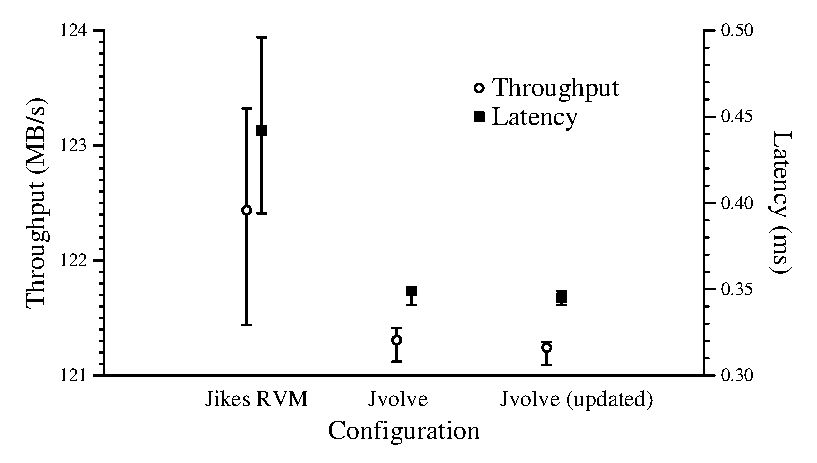
\includegraphics{graphs/jetty-throughput-latency}}
\caption{Throughput and latency measurements of Jetty webserver v5.1.6\label{fig:jetty}}
\end{center}
\end{figure}

\begin{table*}[t]
\begin{footnotesize}
\begin{center}
\begin{tabular}{|r|r|rrrrrrrrrrr|}
                                                                                                                                   \hline
\multirow{2}{*}{\# objects}     & \multicolumn{1}{c}{Heap}   & \multicolumn{11}{|c|}{Fraction of updated objects \T}            \\
                                & \multicolumn{1}{c|}{size}  &
                       0\%  &   10\%  &   20\%  &   30\%  &   40\%  &   50\%  &   60\%  &   70\%  &   80\%  &   90\%  &  100\%  \\ \hline
\multicolumn{13}{|c|}{Garbage collection time (ms) \T}                                                                          \\ \hline \T
 280000 &  160 MB &    78.2 &    81.3 &    83.1 &    89.3 &    99.0 &   103.2 &   108.3 &   113.2 &   113.3 &   120.3 &   120.0 \\
 770000 &  320 MB &   148.9 &   165.0 &   181.9 &   195.8 &   213.2 &   223.2 &   237.0 &   249.0 &   262.0 &   269.5 &   278.6 \\
1760000 &  640 MB &   313.3 &   347.7 &   382.9 &   416.0 &   449.8 &   478.9 &   506.8 &   534.0 &   558.8 &   583.7 &   601.5 \\
3670000 & 1280 MB &   615.4 &   694.6 &   763.0 &   833.6 &   900.1 &   965.9 &  1019.0 &  1076.4 &  1129.9 &  1181.2 &  1217.5 \\ \hline
\multicolumn{13}{|c|}{Running transformation functions (ms) \T}                                                                 \\ \hline \T
 280000 &  160 MB &     0.1 &    13.0 &    23.2 &    34.6 &    43.9 &    54.0 &    62.7 &    74.5 &    84.1 &    93.9 &   104.2 \\
 770000 &  320 MB &     0.1 &    33.7 &    63.1 &    91.2 &   116.8 &   145.4 &   173.9 &   201.0 &   231.3 &   262.0 &   292.6 \\
1760000 &  640 MB &     0.1 &    77.9 &   143.9 &   207.7 &   269.5 &   333.7 &   397.6 &   464.0 &   534.6 &   604.5 &   674.9 \\
3670000 & 1280 MB &     0.1 &   160.8 &   299.2 &   429.4 &   560.2 &   693.8 &   827.3 &   975.0 &  1119.6 &  1263.7 &  1405.4 \\ \hline
\multicolumn{13}{|c|}{Total DSU pause time (ms) \T}                                                                             \\ \hline \T
 280000 &  160 MB &    82.8 &    99.0 &   109.5 &   128.0 &   147.6 &   161.2 &   174.5 &   192.8 &   202.5 &   218.8 &   228.1 \\
 770000 &  320 MB &   153.6 &   202.9 &   249.0 &   291.4 &   334.5 &   372.6 &   414.8 &   455.4 &   498.1 &   535.3 &   576.8 \\
1760000 &  640 MB &   316.6 &   429.5 &   530.5 &   627.2 &   723.4 &   816.0 &   908.6 &  1002.6 &  1097.5 &  1191.5 &  1281.2 \\
3670000 & 1280 MB &   618.7 &   859.0 &  1065.9 &  1269.9 &  1466.1 &  1663.6 &  1850.8 &  2054.2 &  2253.1 &  2448.5 &  2627.9 \\ \hline
\end{tabular}
\end{center}
\end{footnotesize}
\caption{Microbenchmark results: \DSU{} update pause time (in ms) for various heap sizes}
\label{tab:microbench}
\end{table*}


\subsection{Performance}
\label{subsec:performance}

The main performance impact of \DSU{} is the cost of applying an update;
once updated, the application eventually runs without further overhead.  To confirm
%MWH: added "eventually" here because of the cost of recompilation.
%We don't actually measure this though.  Is that a problem?
this claim, we measured the throughput and latency of two Jetty versions while running on
stock \JikesRVM{} and on \DSU{} after dynamically updating to the next version. The performance of these configurations is
essentially identical.

% We report
% on this experiment in Section~\ref{subsec:jetty-perf}.

The cost of applying an update is the time to load any new classes, invoke a
full heap garbage collection, and to apply the transformation methods on
objects belonging to updated classes.
Roughly,
the time to suspend threads and check
that the application is in a safe-point is less than a millisecond, and classloading
time is usually less than 20ms.
% (Classloading could occur in parallel with normal execution.) 
Therefore the update disruption time is primarily
due to the GC and object transformers, and is proportional
to the size of the heap and the fraction of objects being transformed.  We
wrote a simple microbenchmark to measure these overheads.
% Section~\ref{subsec:microbench}
This experiment shows that object
transformation is the dominant cost.

We conducted all our experiments on an Intel Core 2 Quad machine running at 2.4 GHz machine with 2 GB of RAM.
The machine ran Ubuntu 7.10 on Linux kernel version 2.6.22. We implemented
\DSU{} on top of \JRVMVersion{}.

% We also have microbenchmarks where we compare the
% overhead added as a result of running the transformer function.

% \begin{figure}[t]
\begin{small}
\begin{center}
\begin{tabular}{|l|c|c|c|c|} \hline \T
Config.                & \multicolumn{2}{c|}{Throughput (MB/s)}  & \multicolumn{2}{c|}{Latency (ms)} \\ \cline{2-5}
                       & Median   & Quartiles \T                 & Median & Quartiles                \\ \hline \T
\JikesRVM{}            & 122.437  & 121.44--123.32               & 0.442  & 0.394--0.496             \\
\DSU{}                 & 121.308  & 121.12--121.41               & 0.349  & 0.341--0.351             \\
\DSU{} upd             & 121.242  & 121.09--121.29               & 0.345  & 0.341--0.349             \\ \hline
\end{tabular}
\end{center}
\end{small}
% \caption{Throughput and latency measurements for Jetty webserver v5.1.6
% showing median and semi-interquartile range\label{tab:jetty}}
\begin{center}
\scalebox{0.63}{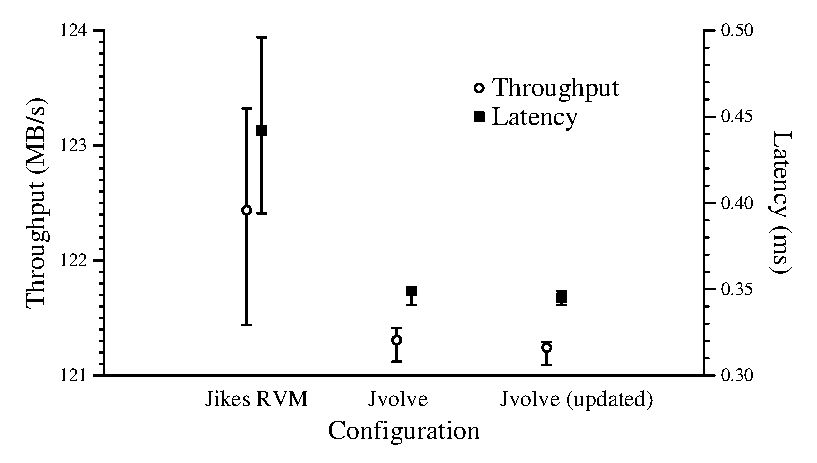
\includegraphics{graphs/jetty-throughput-latency}}
\caption{Throughput and latency measurements of Jetty webserver v5.1.6\label{fig:jetty}}
\end{center}
\end{figure}

% \begin{figure}[t]
\begin{center}
\scalebox{0.63}{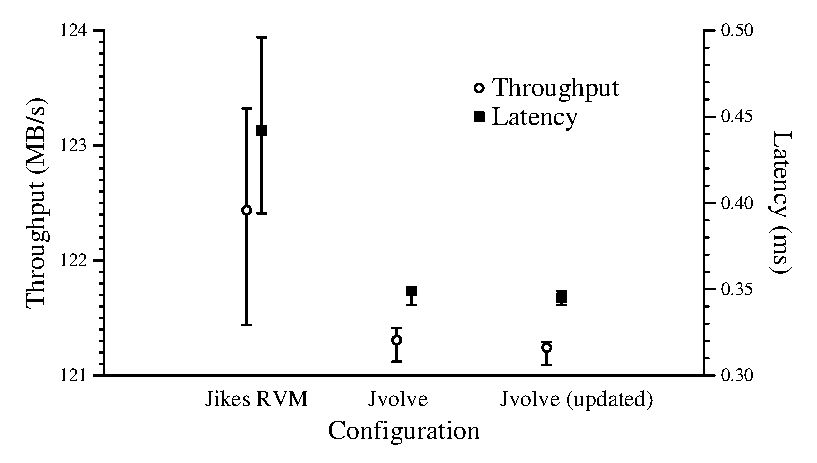
\includegraphics{graphs/jetty-throughput-latency}}
\caption{Throughput and latency measurements of Jetty webserver v5.1.6\label{fig:jetty}}
\end{center}
\end{figure}

% \begin{table*}[t]
\begin{footnotesize}
\begin{center}
\begin{tabular}{|r|r|rrrrrrrrrrr|}
                                                                                                                                   \hline
\multirow{2}{*}{\# objects}     & \multicolumn{1}{c}{Heap}   & \multicolumn{11}{|c|}{Fraction of updated objects \T}            \\
                                & \multicolumn{1}{c|}{size}  &
                       0\%  &   10\%  &   20\%  &   30\%  &   40\%  &   50\%  &   60\%  &   70\%  &   80\%  &   90\%  &  100\%  \\ \hline
\multicolumn{13}{|c|}{Garbage collection time (ms) \T}                                                                          \\ \hline \T
 280000 &  160 MB &    78.2 &    81.3 &    83.1 &    89.3 &    99.0 &   103.2 &   108.3 &   113.2 &   113.3 &   120.3 &   120.0 \\
 770000 &  320 MB &   148.9 &   165.0 &   181.9 &   195.8 &   213.2 &   223.2 &   237.0 &   249.0 &   262.0 &   269.5 &   278.6 \\
1760000 &  640 MB &   313.3 &   347.7 &   382.9 &   416.0 &   449.8 &   478.9 &   506.8 &   534.0 &   558.8 &   583.7 &   601.5 \\
3670000 & 1280 MB &   615.4 &   694.6 &   763.0 &   833.6 &   900.1 &   965.9 &  1019.0 &  1076.4 &  1129.9 &  1181.2 &  1217.5 \\ \hline
\multicolumn{13}{|c|}{Running transformation functions (ms) \T}                                                                 \\ \hline \T
 280000 &  160 MB &     0.1 &    13.0 &    23.2 &    34.6 &    43.9 &    54.0 &    62.7 &    74.5 &    84.1 &    93.9 &   104.2 \\
 770000 &  320 MB &     0.1 &    33.7 &    63.1 &    91.2 &   116.8 &   145.4 &   173.9 &   201.0 &   231.3 &   262.0 &   292.6 \\
1760000 &  640 MB &     0.1 &    77.9 &   143.9 &   207.7 &   269.5 &   333.7 &   397.6 &   464.0 &   534.6 &   604.5 &   674.9 \\
3670000 & 1280 MB &     0.1 &   160.8 &   299.2 &   429.4 &   560.2 &   693.8 &   827.3 &   975.0 &  1119.6 &  1263.7 &  1405.4 \\ \hline
\multicolumn{13}{|c|}{Total DSU pause time (ms) \T}                                                                             \\ \hline \T
 280000 &  160 MB &    82.8 &    99.0 &   109.5 &   128.0 &   147.6 &   161.2 &   174.5 &   192.8 &   202.5 &   218.8 &   228.1 \\
 770000 &  320 MB &   153.6 &   202.9 &   249.0 &   291.4 &   334.5 &   372.6 &   414.8 &   455.4 &   498.1 &   535.3 &   576.8 \\
1760000 &  640 MB &   316.6 &   429.5 &   530.5 &   627.2 &   723.4 &   816.0 &   908.6 &  1002.6 &  1097.5 &  1191.5 &  1281.2 \\
3670000 & 1280 MB &   618.7 &   859.0 &  1065.9 &  1269.9 &  1466.1 &  1663.6 &  1850.8 &  2054.2 &  2253.1 &  2448.5 &  2627.9 \\ \hline
\end{tabular}
\end{center}
\end{footnotesize}
\caption{Microbenchmark results: \DSU{} update pause time (in ms) for various heap sizes}
\label{tab:microbench}
\end{table*}


\paragraph{Jetty performance.}
To see the effect of updating on application performance, we measured Jetty
under various configurations using httperf, a webserver
benchmarking tool.\footnote{\url{http://www.hpl.hp.com/research/linux/httperf}}  We used httperf to issue roughly 800 new connection
requests/second, which we observed to be Jetty's saturation rate.
Each connection makes 5 serial requests for a 40 Kbyte file. Httperf
reports average throughput and average per-request latency over a 60 second period. We
ran this experiment 21 times and report the median and
quartiles of the throughput and latency reports. With 21 runs, the range between
the quartiles serves as a 98\% confidence interval~\cite{PrattGibbons81}.
In order to eliminate network traffic
effects, we ran the server on two cores of a quad-core machine and the
client on another core.

Figure~\ref{fig:jetty} shows our results in tabular form and plotted graphically.  The second and third columns
of the table
report the median throughput and the range between the two quartiles.
The third column and fourth column report the median latency and the
inter-quartile range.  The
first and seconds rows illustrate the performance of Jetty version 5.1.6
running on stock \JikesRVM{} and \DSU, respectively. The third row shows
the performance on \DSU{} of Jetty 5.1.6 dynamically updated from version
5.1.5 prior to the start of the experiment.
% \todo{Find a way to introduce the graph} Figure~\ref{fig:jetty} plots the results shown in the table.
The performance of the two \DSU{} configurations
is essentially identical: the two configurations' corresponding
inter-quartile ranges largely overlap.
The performance of \DSU{} is also quite similar to the performance of
stock \JikesRVM.  There are many small differences between \DSU{} and the stock
implementation that change VM code size, code layout, and garbage
collection behavior.  These differences may impact performance
directly and they may indirectly affect other elements of the VM,
such as the timing of garbage collections and JIT
optimizations (such indirect effects make VMs notoriously difficult to
benchmark~\cite{dacapo-cacm}).


%%% Local Variables: 
%%% mode: latex
%%% TeX-master: "../pldi64"
%%% End: 

% \begin{table*}[t]
\begin{footnotesize}
\begin{center}
\begin{tabular}{|r|r|rrrrrrrrrrr|}
                                                                                                                                   \hline
\multirow{2}{*}{\# objects}     & \multicolumn{1}{c}{Heap}   & \multicolumn{11}{|c|}{Fraction of updated objects \T}            \\
                                & \multicolumn{1}{c|}{size}  &
                       0\%  &   10\%  &   20\%  &   30\%  &   40\%  &   50\%  &   60\%  &   70\%  &   80\%  &   90\%  &  100\%  \\ \hline
\multicolumn{13}{|c|}{Garbage collection time (ms) \T}                                                                          \\ \hline \T
 280000 &  160 MB &    78.2 &    81.3 &    83.1 &    89.3 &    99.0 &   103.2 &   108.3 &   113.2 &   113.3 &   120.3 &   120.0 \\
 770000 &  320 MB &   148.9 &   165.0 &   181.9 &   195.8 &   213.2 &   223.2 &   237.0 &   249.0 &   262.0 &   269.5 &   278.6 \\
1760000 &  640 MB &   313.3 &   347.7 &   382.9 &   416.0 &   449.8 &   478.9 &   506.8 &   534.0 &   558.8 &   583.7 &   601.5 \\
3670000 & 1280 MB &   615.4 &   694.6 &   763.0 &   833.6 &   900.1 &   965.9 &  1019.0 &  1076.4 &  1129.9 &  1181.2 &  1217.5 \\ \hline
\multicolumn{13}{|c|}{Running transformation functions (ms) \T}                                                                 \\ \hline \T
 280000 &  160 MB &     0.1 &    13.0 &    23.2 &    34.6 &    43.9 &    54.0 &    62.7 &    74.5 &    84.1 &    93.9 &   104.2 \\
 770000 &  320 MB &     0.1 &    33.7 &    63.1 &    91.2 &   116.8 &   145.4 &   173.9 &   201.0 &   231.3 &   262.0 &   292.6 \\
1760000 &  640 MB &     0.1 &    77.9 &   143.9 &   207.7 &   269.5 &   333.7 &   397.6 &   464.0 &   534.6 &   604.5 &   674.9 \\
3670000 & 1280 MB &     0.1 &   160.8 &   299.2 &   429.4 &   560.2 &   693.8 &   827.3 &   975.0 &  1119.6 &  1263.7 &  1405.4 \\ \hline
\multicolumn{13}{|c|}{Total DSU pause time (ms) \T}                                                                             \\ \hline \T
 280000 &  160 MB &    82.8 &    99.0 &   109.5 &   128.0 &   147.6 &   161.2 &   174.5 &   192.8 &   202.5 &   218.8 &   228.1 \\
 770000 &  320 MB &   153.6 &   202.9 &   249.0 &   291.4 &   334.5 &   372.6 &   414.8 &   455.4 &   498.1 &   535.3 &   576.8 \\
1760000 &  640 MB &   316.6 &   429.5 &   530.5 &   627.2 &   723.4 &   816.0 &   908.6 &  1002.6 &  1097.5 &  1191.5 &  1281.2 \\
3670000 & 1280 MB &   618.7 &   859.0 &  1065.9 &  1269.9 &  1466.1 &  1663.6 &  1850.8 &  2054.2 &  2253.1 &  2448.5 &  2627.9 \\ \hline
\end{tabular}
\end{center}
\end{footnotesize}
\caption{Microbenchmark results: \DSU{} update pause time (in ms) for various heap sizes}
\label{tab:microbench}
\end{table*}

\begin{figure}[t]
\begin{center}
\scalebox{0.69}{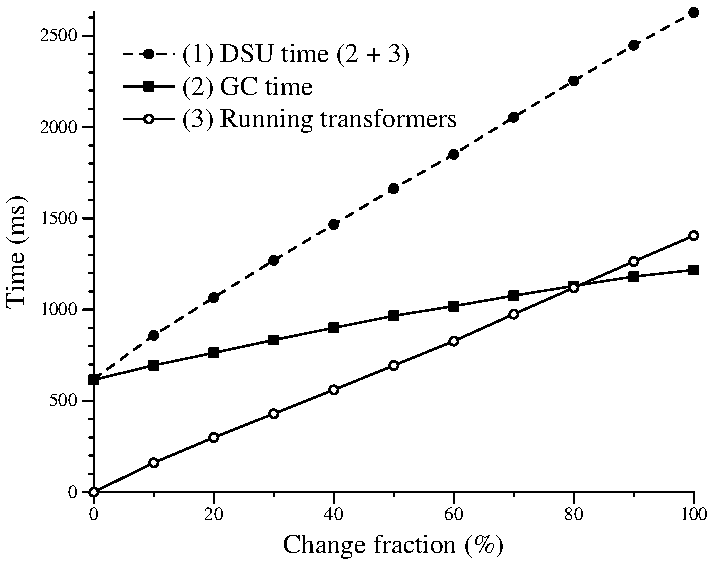
\includegraphics{graphs/microbench}}
\caption{Microbenchmark pause times with a heap size of 1280 MB containing
3.67 million objects\label{fig:microbench}}
\end{center}
\end{figure}


\paragraph{Microbenchmarks.}
The two dominant factors that determine \DSU{} update time are the time to
perform a GC, determined by the number of objects, and the time to run
object transformers, determined by the fraction of objects being
updated.  To measure the cost of each, we devised a simple 
microbenchmark that creates an array of objects and transforms a specified
fraction of these objects when a \DSU{} update is triggered. The
microbenchmark has two simple classes, \texttt{Change} and
\texttt{NoChange}. Both contain three integer fields, and three reference
fields that are always {\tt null}. The update adds an integer field to
{\tt Change}. The user-provided object transformation function copies the
existing fields and initializes the new field to zero.
% The benchmark contains two arrays,
% one for \texttt{Change} objects and one for \texttt{NoChange} objects.
We measure the cost of performing an update while varying the total
number of objects and the fraction of objects of each type. The number of
objects is the maximum that can fit in heap sizes 32, 64, 128 and 256
MB.  Note that \JikesRVM{}'s heap includes VM data structures as well. We
measure the running time in a generous heap, five times the minimum required size, such that the only collections are those DSU triggers. We report the
median of 21 runs.

Table~\ref{tab:microbench} shows the elapsed time
while varying the number of total objects and the fraction of the objects that are updated.  The
variance was insignificant, so we do not report it.   % KSM: I deleted the first row, since it is the only one with this problem, which is due to other costs dominating, e.g., stack walking etc. because apparently copying 40,000 objects takes no time at all. \todo{some of the
%   results are unintuitive; e.g., the time goes down as you move to the
%   right, sometimes.  Make a comment here about that being the way of
%   things with sophisticated machines?  Can't blame it on the
%   variance.}
The first group of rows reports
garbage collection time, the second group reports the time to transform
all updated objects, and the final group reports the total update time, which
includes the sum of the GC and transformation time, the time to load and install the updated classes, synchronize
running threads, and find a DSU safe point. 
The first column of the table shows the number of objects in the test, and
the second column the heap size. Columns 3 though 13 show pause times for
varying fractions (from 0\% to 100\%) of updated objects. 
% Looking at
% the last column of the table, we can see that the GC time results
% (first group of rows) for
% various heap sizes are roughly the same as the transformation time
% results (second group of rows), showing the time to transform an
% object to be roughly equal to the time to copy an object in the collector.

To shed light on the results in the table,
Figure~\ref{fig:microbench} plots collection time, transformer time and
total update time for the microbenchmark with 3.67 million objects in a
1280 MB heap.  The figure shows that the costs of garbage collection and
transformation increase  as a function of the number of changed objects.  The slope of the ``GC time'' line illustrates the cost to deal
with an increasing number of transformed objects.  This cost includes
creating an additional copy of each transformed object; creating the
update log entry with a pointer to the old and new copy; and caching a
pointer to the old copy from the new copy.  The slope of the
``Running transformers'' line illustrates the added cost of iterating
over the update log and actually running the transformers.  This extra
processing to handle transforming objects increases the total pause
time with all objects updated by roughly four times compared to the
pause time with no object updated.  The ``Running
Transformers'' line is steeper than the ``GC time'' line, revealing that
the cost of running transformers is higher than the extra copying cost
incurred during GC\@.

Transformations are more expensive than standard copying GC. The GC uses
\texttt{memcopy}, which is highly optimized, whereas our transformer
functions use reflection to look up \texttt{jvolveObject}, and this
function copies one field at a time.  One optimization would be to eliminate the log by copying
the old and new objects to their own space and % appending to each one a
% pointer to their corresponding new object.
walking through and transforming each object.
The cost of reflection could be
reduced by caching the lookup, but even then a na\"ively compiled
field-by-field copy is much slower than the collector's
highly-optimized copying loop.  % Another possible optimization is to
% specially compile transformers to replace idiomatic use of copying
% assignments to contiguous fields by a \texttt{memcopy} over the
% corresponding range.


%%% Local Variables: 
%%% mode: latex
%%% TeX-master: "../pldi64"
%%% End: 

